\documentclass{poly}
\usepackage{main}

\title{Chapitre 8 : Trigonométrie}
\author{Première Spécialité Mathématique}
\date{}

\begin{document}
\maketitle
\section{Cercle trigonométrique : Mesure d'angle}
\begin{definition}
Soit $(O;I;J)$ un repère orthonormée. Le \textbf{cercle trigonométrique} est le cercle de centre $O$ et de rayon $OI = 1$. Le cercle est muni d'une orientation :
\begin{itemize}
\item Le sens direct ou trigonométrique est le sens antihoraire;
\item Le sens indirect est le sens horaire.
\end{itemize}
\end{definition}
\begin{center}
\begin{tikzpicture}
\draw[help lines] (-4.25,-4.25) grid[step=0.5] (4.25,4.25);
\draw[axis] (-4.25,0) -- (4.25,0) node[right] {$x$}; 
\draw[axis] (0,-4.25) -- (0,4.25) node[above] {$y$};
\draw (0,0) node[below left] {$O$}; 
\draw (3,-0.1) -- (3,0.1) node[above right] {$I$}; 
\draw (0.1,3) -- (-0.1,3) node[above left] {$J$};
\draw (0,0) circle (3);
\draw[->] (3.46,2) arc (30:80:4) node[above] {$+$};
\end{tikzpicture}
\end{center}
\begin{remark}
Le but du cercle trigonométrique est de définir une notion de mesure d'angle \og universelle \fg.
\end{remark}
\newpage
\begin{definition}
Soit $M$ un point du cercle trigonométrique. Sa position est entièrement déterminée par l'angle formé par les demi-droites $[OI)$ et $[OM)$.

Une mesure de l'angle est donnée par la longueur d'un parcours sur le cercle partant de $I$ et arrivant à $M$. Cette mesure est positive si le chemin a été parcouru dans le sens trigonométrique, négative sinon. L'unité de mesure est le \textbf{radian}.
\end{definition}
\begin{center}
\begin{tikzpicture}
\draw[help lines] (-4.25,-4.25) grid[step=0.5] (4.25,4.25);
\draw[axis] (-4.25,0) -- (4.25,0) node[right] {$x$}; 
\draw[axis] (0,-4.25) -- (0,4.25) node[above] {$y$};
\draw (0,0) node[below left] {$O$}; 
\draw (3,-0.1) -- (3,0.1) node[above right] {$I$}; 
\draw (0.1,3) -- (-0.1,3) node[above left] {$J$};
\draw (0,0) circle (3);
\draw[->] (3.46,2) arc (30:80:4) node[above] {$+$};
\draw (50:3) node {$\bullet$} node[above right] {$M$};
\draw (0,0) -- (50:3);
\draw[ultra thick] (3,0) arc (0:50:3);
\draw[->] (1,0) arc (0:50:1) node[midway, right] {$\alpha$};
\end{tikzpicture}
\end{center}
\begin{remark}
Il y a une infinité de parcours partant de $I$ et arrivant à $M$. Il suffit d'ajouter un certain nombre de tours complets du cercle.

Il y a donc une infinité de mesure d'angle possible pour un même angle.
\end{remark}
\begin{proposition}
Soit un angle dont une des mesures en radian est $\alpha$. Alors, les autres mesures de cet angle sont de la forme $\alpha + 2k\pi$ avec $k \in \Z$.

Seule une seule de ces mesures est dans l'intervalle $]-\pi;\pi]$: on l'appelle \textbf{mesure principale} de l'angle. 
\end{proposition}
\begin{remark} Ce tableau répertorie les mesures principales d'angle classique en radian.
\begin{equation*}
\begin{tblr}{hlines, vlines, cells={mode=dmath}}
\text{Degré} & \qty{0}{\degree} & \qty{30}{\degree} & \qty{45}{\degree} & \qty{60}{\degree} & \qty{90}{\degree} & \qty{180}{\degree} & \qty{270}{\degree} & \qty{360}{\degree}\\
\text{Radian}& 0 & \dfrac{\pi}{6} & \dfrac{\pi}{4} & \dfrac{\pi}{3} & \dfrac{\pi}{2} & \pi & \dfrac{3\pi}{2} & 2\pi
\end{tblr}
\end{equation*}
\end{remark}
\newpage
\section{Sinus et Cosinus}
\subsection{Définition}
\begin{definition}
Soit $\alpha$ un nombre réel. On note $M$ un point du cercle trigonométrique tel que $\alpha$ est une mesure en radians de l'angle orienté $\widehat{IOM}$. Alors,
\begin{itemize}
\item le cosinus de $\alpha$, noté $\cos(\alpha)$, est défini comme étant \textbf{l'abscisse} du point $M$;
\item le sinus de $\alpha$, noté $\sin(\alpha)$, est défini comme étant \textbf{l'ordonnée} du point $M$.
\end{itemize}
\end{definition}
\begin{center}
\begin{tikzpicture}[scale=0.8]
\draw[help lines] (-4.25,-4.25) grid[step=0.5] (4.25,4.25);
\draw[axis] (-4.25,0) -- (4.25,0) node[right] {$x$}; 
\draw[axis] (0,-4.25) -- (0,4.25) node[above] {$y$};
\draw (0,0) node[below left] {$O$}; 
\draw (3,-0.1) -- (3,0.1) node[above right] {$I$}; 
\draw (0.1,3) -- (-0.1,3) node[above left] {$J$};
\draw (0,0) circle (3);
\draw[->] (3.46,2) arc (30:80:4) node[above] {$+$};
\draw (50:3) node {$\bullet$} node[above right] {$M$};
\draw (0,0) -- (50:3);
\draw[ultra thick] (3,0) arc (0:50:3);
\draw[->] (1,0) arc (0:50:1) node[midway, right] {$\alpha$};
\draw[dashed] (50:3) -- ({3*cos(50)},0) node {$\bullet$} node[below] {$\cos(\alpha)$};
\draw[dashed] (50:3) -- (0,{3*sin(50)}) node {$\bullet$} node[left] {$\sin(\alpha)$};
\end{tikzpicture}
\end{center}
\begin{center}
\begin{tikzpicture}[scale=0.8]
\draw[help lines] (-0.25,-0.25) grid[step=1] (8.25,8.25);
\draw[axis] (-0.25,0) -- (8.25,0) node[right] {$x$};
\draw[axis] (0,-0.25) -- (0,8.25) node[above] {$y$};
\draw (0,0) -- (50:8) node {$\bullet$} node[above right] {$M$} node[midway,above] {$1$};
\draw[ultra thick] (8,0) arc (0:50:8);
\draw[->] (2,0) arc (0:50:2) node[midway,right] {$\alpha$};
\draw[dashed] (50:8) -- ({8*cos(50)},0) node[midway,right] {$\sin(\alpha)$}; 
\draw[dashed] (50:8) -- (0,{8*sin(50)}) node[midway,above] {$\cos(\alpha)$};
\draw[ultra thick] (0,0) -- ({8*cos(50)},0) node[midway,below] {$\cos(\alpha)$};
\draw[ultra thick] (0,0) -- (0,{8*sin(50)}) node[midway,left] {$\sin(\alpha)$};
\draw ({8*cos(50)},0) ++ (-0.5,0) -- ++ (0,0.5) -- ++ (0.5,0);
\clip (-0.25,-0.25) rectangle (8.25,8.25);
\draw (0,0) circle (8);
\end{tikzpicture}
\end{center}
\begin{theorem}
Soit $\alpha$ un nombre réel. Alors,
\begin{equation*}
(\cos(\alpha))^2 + (\sin(\alpha))^2 = 1 
\end{equation*}
\end{theorem}
\newpage
\subsection{Valeurs remarquables}
\begin{minipage}{0.45\textwidth}
\subsubsection{$\alpha = \dfrac{\pi}{4}$}
\begin{center}
\begin{tikzpicture}[scale=0.7]
\draw[help lines] (-0.25,-0.25) grid[step=1] (8.25,8.25);
\draw[axis] (-0.25,0) -- (8.25,0) node[right] {$x$};
\draw[axis] (0,-0.25) -- (0,8.25) node[above] {$y$};
\draw (0,0) -- (45:8) node {$\bullet$} node[above right] {$M$};
\draw[ultra thick] (8,0) arc (0:45:8);
\draw[->] (1.5,0) arc (0:45:1.5) node[midway,right] {$\dfrac{\pi}{4}$};
\draw[dashed] (45:8) -- ({8*cos(45)},0) node[midway,right] {$\sin(\alpha)$} node[midway,sloped] {$//$}; 
\draw (0,0) -- ({8*cos(45)},0) node[midway,below] {$\cos(\alpha)$} node[midway] {$//$};
\draw ({8*cos(45)},0) ++ (-0.5,0) -- ++ (0,0.5) -- ++ (0.5,0);
\clip (-0.25,-0.25) rectangle (8.25,8.25);
\draw (0,0) circle (8);
\end{tikzpicture}
\end{center}
\begin{equation*}
\begin{cases}
\cos(\alpha) = \sin(\alpha)\\
(cos(\alpha))^2 + (sin(\alpha))^2 = 1
\end{cases}
\end{equation*}
\end{minipage}
\hfill\vline\hfill
\begin{minipage}{0.45\textwidth}
\subsubsection{$\alpha = \dfrac{\pi}{3}$}
\begin{center}
\begin{tikzpicture}[scale=0.7]
\draw[help lines] (-0.25,-0.25) grid[step=1] (8.25,8.25);
\draw[axis] (-0.25,0) -- (8.25,0) node[right] {$x$};
\draw[axis] (0,-0.25) -- (0,8.25) node[above] {$y$};
\draw (0,0) -- (60:8) node {$\bullet$} node[above right] {$M$} -- (8,0);
\draw[ultra thick] (8,0) arc (0:60:8);
\draw[->] (1,0) arc (0:60:1) node[midway,right] {$\dfrac{\pi}{3}$};
\draw[dashed] (60:8) -- ({8*cos(60)},0) node[midway,right] {$\sin(\alpha)$};
\draw (0,0) -- ({8*cos(60)},0) node[midway,below] {$\cos(\alpha)$} node[midway] {$//$} -- (8,0) node[midway,below] {$\cos(\alpha)$} node[midway] {$//$};
\draw ({8*cos(60)},0) ++ (-0.5,0) -- ++ (0,0.5) -- ++ (0.5,0);
\clip (-0.25,-0.25) rectangle (8.25,8.25);
\draw (0,0) circle (8);
\end{tikzpicture}
\end{center}
\begin{equation*}
\begin{cases}
2cos(\alpha) = 1\\
(cos(\alpha))^2 + (sin(\alpha))^2 = 1
\end{cases}
\end{equation*}
\end{minipage}
\begin{remark}
En résolvant ces \og problèmes de géométrie \fg, on en déduit ces valeurs particulières de $\cos(\alpha)$ et $\sin(\alpha)$. C'est comme cela que l'on obtient le tableau suivant :
\begin{equation*}
\begin{tblr}{hlines, vlines, cells={mode=dmath,c}, stretch=0, rows={ht=\baselineskip}}
\alpha \text{ (en Degrés)} & \qty{0}{\degree} & \qty{30}{\degree} & \qty{45}{\degree} & \qty{60}{\degree} & \qty{90}{\degree}\\
\alpha \text{ (en Radians)}& 0 & \frac{\pi}{6} & \frac{\pi}{4} & \frac{\pi}{3} & \frac{\pi}{2}\\
\sin(\alpha)&0&\frac{1}{2}&\frac{\sqrt{2}}{2}&\frac{\sqrt{3}}{2}&1\\
\cos(\alpha)&1&\frac{\sqrt{3}}{2}&\frac{\sqrt{2}}{2}&\frac{1}{2}&0\\
\end{tblr}
\end{equation*}
\begin{tcolorbox}
La méthode pour reproduire les deux dernières lignes du tableau est la suivante :
\begin{enumerate}
\item On commence avec la ligne $\sin(\alpha)$;
\item On numérote les cases dans l'ordre de gauche à droite en partant de $0$ : $0; 1; 2; 3; 4$;
\item On divise chaque case par $2$;
\item On prend la racine carrée du numérateur;
\item On simplifie ce qu'il y a à simplifier (par exemple, $\sqrt{4} = 2$)
\item Pour la ligne $\cos(\alpha)$, on reproduit la ligne $\sin(\alpha)$ mais de droite à gauche\dots
\end{enumerate}
\end{tcolorbox}
\end{remark}
\newpage
\section{Fonctions sinus et cosinus}
\subsection{Définition et courbes représentatives}
À chaque nombre réel $x$ l'on peut associer un sinus $\sin(x)$ et un cosinus $\cos(x)$, le sinus et le cosinus peuvent donc être considérées comme des fonctions.
\begin{definition}
\hfill
\begin{itemize}
\item La fonction \textbf{sinus} est la fonction définie par:
\begin{equation*}
\function{\sin}{\R}{[-1;1]}{x}{\sin(x)}
\end{equation*} 
\item La fonction \textbf{cosinus} est la fonction définie par:
\begin{equation*}
\function{\cos}{\R}{[-1;1]}{x}{\cos(x)}
\end{equation*} 
\end{itemize}
\end{definition}
\begin{proposition}
Les courbes représentatives des fonctions sinus et cosinus sont données par :
\vspace*{0.25cm}

\begin{minipage}{0.45\textwidth}
\begin{center}
\begin{equation*}
x \mapsto \sin(x)
\end{equation*}

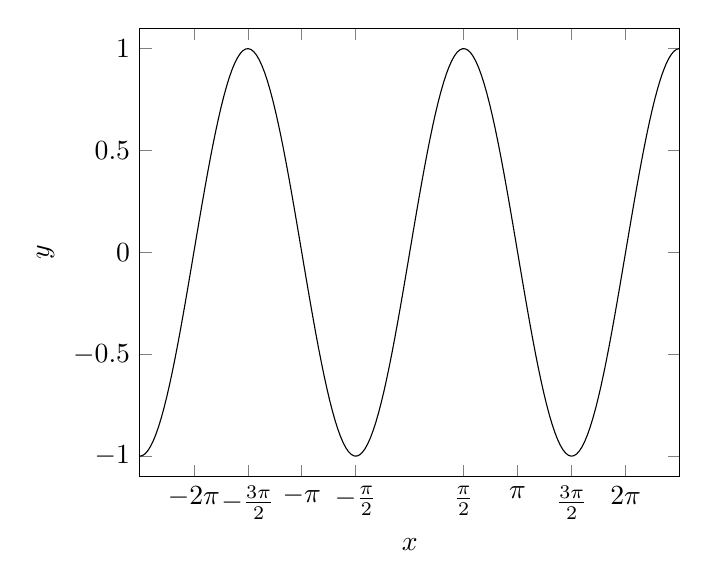
\begin{tikzpicture}
\begin{axis}[
  xmin=-(5/2)*pi,
  xmax=(5/2)*pi,
  ymin=-1.1,
  ymax=1.1,
  xtick={-2*pi, -(3/2)*pi, -pi, -(1/2)*pi, (1/2)*pi, pi, (3/2)*pi, 2*pi},
  xticklabels={$-2\pi$, $-\frac{3\pi}{2}$, $-\pi$, $-\frac{\pi}{2}$, $\frac{\pi}{2}$, $\pi$, $\frac{3\pi}{2}$, $2\pi$},
  xlabel={$x$},
  ylabel={$y$},
  ]
\addplot[domain=-(5/2)*pi:(5/2)*pi,samples=200]{sin(deg(x))};
\end{axis}
\end{tikzpicture}
\end{center}  
\end{minipage}
\hfill\vline\hfill
\begin{minipage}{0.45\textwidth}
\begin{center}
\begin{equation*}
x \mapsto \cos(x)
\end{equation*}

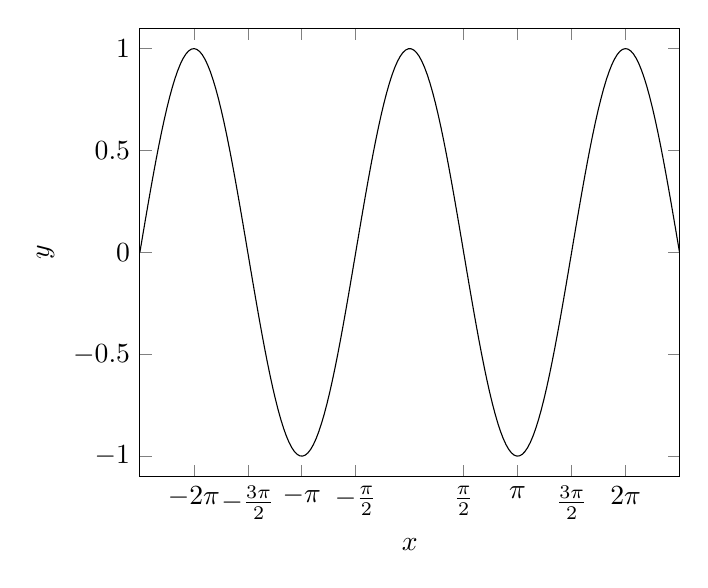
\begin{tikzpicture}
\begin{axis}[
  xmin=-(5/2)*pi,
  xmax=(5/2)*pi,
  ymin=-1.1,
  ymax=1.1,
  xtick={-2*pi, -(3/2)*pi, -pi, -(1/2)*pi, (1/2)*pi, pi, (3/2)*pi, 2*pi},
  xticklabels={$-2\pi$, $-\frac{3\pi}{2}$, $-\pi$, $-\frac{\pi}{2}$, $\frac{\pi}{2}$, $\pi$, $\frac{3\pi}{2}$, $2\pi$},
  xlabel={$x$},
  ylabel={$y$},
  ]
\addplot[domain=-(5/2)*pi:(5/2)*pi,samples=200]{cos(deg(x))};
\end{axis}
\end{tikzpicture}
\end{center}
\end{minipage}
\end{proposition}
\newpage
\subsection{Propriétés : Périodicité et Parité}
\begin{proposition}
Les fonctions sinus et cosinus sont $2\pi$-périodiques : pour tout $x$ réels, on a 
\begin{equation*}
sin(x + 2\pi) = sin(x) \quad\mathrm{et}\quad cos(x + 2\pi) = cos(x)
\end{equation*}
\end{proposition}
\begin{remark}
Cette proposition se constate sur les courbes représentatives de ces fonctions : \og les vagues se répètent sur chaque intervalle de taille $2\pi$\fg.
\end{remark}
\begin{proposition}
\hfill
\begin{itemize}
\item La fonction sinus est \textbf{impaire} : pour tout $x$ réel, on a
\begin{equation*}
\sin(-x) = - \sin(x)
\end{equation*}
\item La fonction cosinus est \textbf{paire} : pour tout $x$ réel, on a
\begin{equation*}
\cos(-x) = \cos(x)
\end{equation*}
\end{itemize}
\end{proposition}
\begin{remark}
\begin{itemize}
\item Du point de vue des courbes représentatives, cette propriété est illustrée par le fait que la courbe du sinus admet pour centre de symétrie l'origine du repère, alors que le cosinus admet pour axe de symétrie l'axe des ordonnées.
\item Du point du cercle trigonométrique, cette propriété est la réponse à la question \og Comment se comporte le sinus et le cosinus si l'on parcours le cercle dans le sens indirect (négatif) ? \fg. 
\end{itemize}
\begin{center}
\begin{tikzpicture}
\draw[help lines] (-4.25,-4.25) grid[step=0.5] (4.25,4.25);
\draw[axis] (-4.25,0) -- (4.25,0) node[right] {$x$}; 
\draw[axis] (0,-4.25) -- (0,4.25) node[above] {$y$};
\draw (0,0) node[below left] {$O$}; 
\draw (3,-0.1) -- (3,0.1) node[above right] {$I$}; 
\draw (0.1,3) -- (-0.1,3) node[above left] {$J$};
\draw (0,0) circle (3);
\draw[->] (3.46,2) arc (30:80:4) node[above] {$+$};
\draw (50:3) node {$\bullet$};
\draw (0,0) -- (50:3);
\draw[->] (1,0) arc (0:50:1) node[midway, right] {$\alpha$};
\draw[dashed] (50:3) -- ({3*cos(50)},0) node {$\bullet$} node[above right] {$\cos(\alpha)$};
\draw[dashed] (50:3) -- (0,{3*sin(50)}) node {$\bullet$} node[left] {$\sin(\alpha)$};
\draw (0,0) -- (-50:3);
\draw (-50:3) node {$\bullet$};
\draw[dashed] (-50:3) -- ({3*cos(50)},0);
\draw[dashed] (-50:3) -- (0,{3*sin(-50)}) node {$\bullet$} node[left] {$\sin(-\alpha)$};
\draw[->] (1,0) arc (0:-50:1) node[midway, right] {$-\alpha$};
\end{tikzpicture}
\end{center}

\end{remark}
\end{document}